\chapter{Review of Pertinent Publications}
%\todo[inline]{replace CITEME tags in Development of Rationale and Review of Published Works}

Our previous attempts to infer \glspl{CRE} bioinformatically have been relatively successful.
Comparative genomics by way of the \gls{MDOS} program allowed us to infer a set of k-mers that should represent \glspl{CRE} conserved among three species of mosquitoes (\Aa, \Ag, \Cq).
This method used no expression information in the process of predicting the \glspl{CRE}.
However, we were able to show that a sub-set of the inferred \glspl{CRE} were enriched significantly in abundance profiles derived from a previous affymetrix-based bloodfeeding experiment in \Ag\ \cite{Marinotti2005},\cite{Marinotti2006},\cite{Sieglaff2009}.
Comparing transcriptional abundance profiles between sugarfed and bloodfed (5h \gls{PBM}) \Aa\ mosquitoes allowed us to predict multiple putative \glspl{CRE} when we focused on transcripts that were detected at high levels in in bloodfed mosquitoes but undetectable in sugarfed females \cite{Bonizzoni2011}.
Possible \glspl{CRM} were observed by visual inspection as well, but efforts to confirm biological meaningfulness have not yet been completed.
Putative \glspl{CRM} were again observed by visual inspection in an experiment comparing mRNA abundance profiles between \Aa\ fed with blood infected with dengue virus and those fed with non-infected blood.
In this study, specific tissues were dissected and analyzed separately providing a level of tissue specificity as well.
These \gls{CRM} results also remain in the process of being confirmed experimentally.

These studies have provided useful lessons that I have incorporated into the approach described in Chapter \ref{chap:3}.
A common theme among these lessons is the importance of the relative ratio of signal-to-noise contained in the data-set being examined.
For example, in \citet{Bonizzoni2011}, the most successful \gls{CRE} prediction results arose from a gene-set characterized by a fairly restrictive abundance profile definition (the requirement that transcripts be detected highly at 5h \gls{PBM} but completely undetectable in sugarfed mosquitoes).
This yielded a gene-set of just 40 members.
\citet{bonizzoni2012complex} further demonstrates that \gls{functional genomics} results are sensitive to the definition of gene-sets used for analysis.
In addition to abundance profile definition, \citet{Bonizzoni2011} illustrated that, in \Aa, the official annotation is incomplete and contains at least some level of annotation errors that may be considered particularly troublesome to analyses that rely on accurate definition of putative promoter sequences; however, it also provides support that, despite containing errors, the current state of annotation is sufficient to allow \gls{CRE} prediction.
Finally, in experiments comparing mRNA abundance profiles between three different strains of a single species (\Aa), \citet{bonizzoni2012strain} illustrates the need to take precautions when comparing differences in transcript abundance profiles between species that are estimated to have last shared a common ancestor as long as 200 \gls{Mya}.


\section{Comparative genomics allows the discovery of \textit{cis}-regulatory elements in mosquitoes. \cite{Sieglaff2009}}

\begin{figure}[hp]
\centering

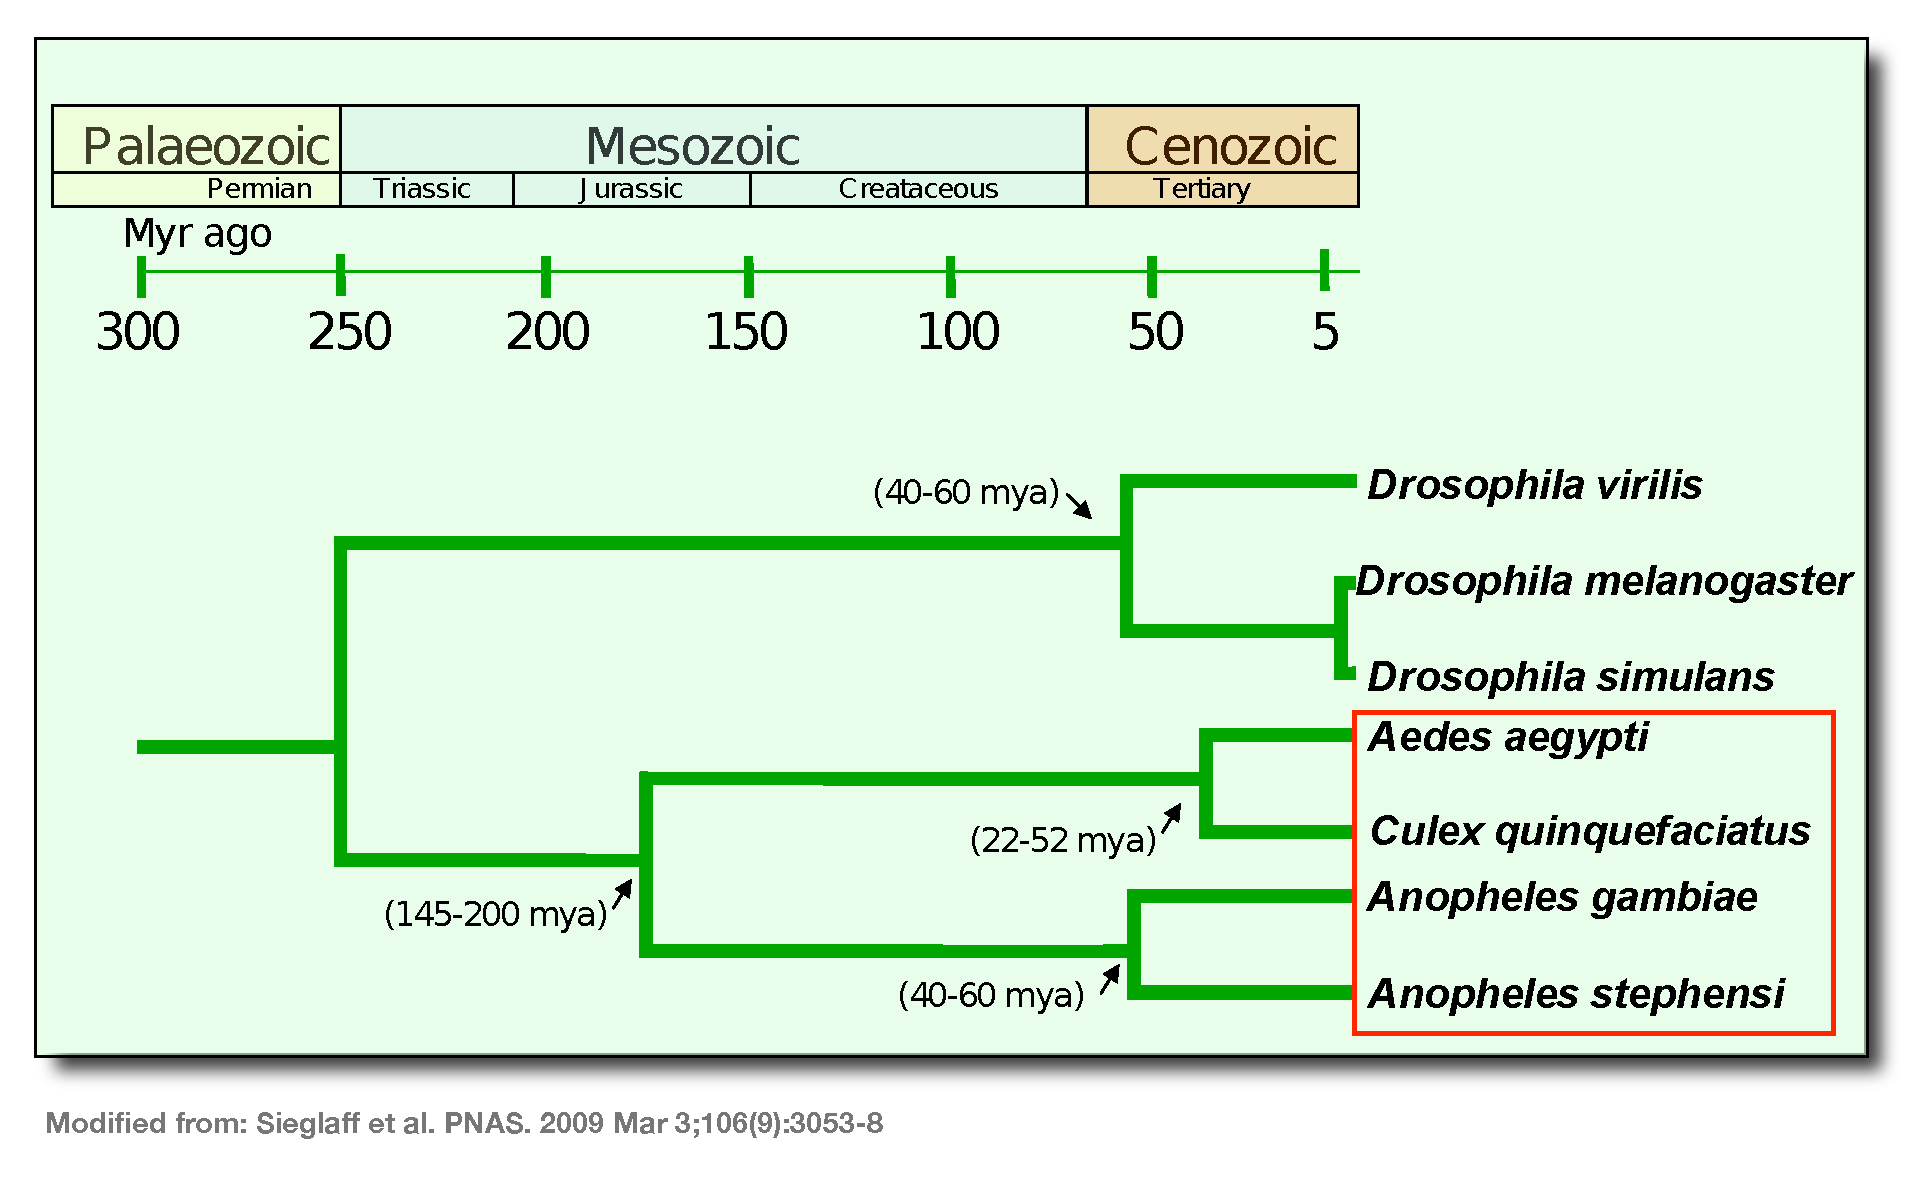
\includegraphics[width=.7\textwidth]{figures/figs/mosqPhyloTree.pdf}

\caption[Phylogenetic relationships between four vector mosquitoes]{\bsf{Phylogenetic relationships between four vector mosquitoes compared with representative \textit{Drosophila} species:} \\ \sf
\dummytext[1]

Adapted from \cite{Sieglaff2009}}
\label{fig:mosqPhyloTree}
\end{figure}

\begin{figure}[hp]

\hfil
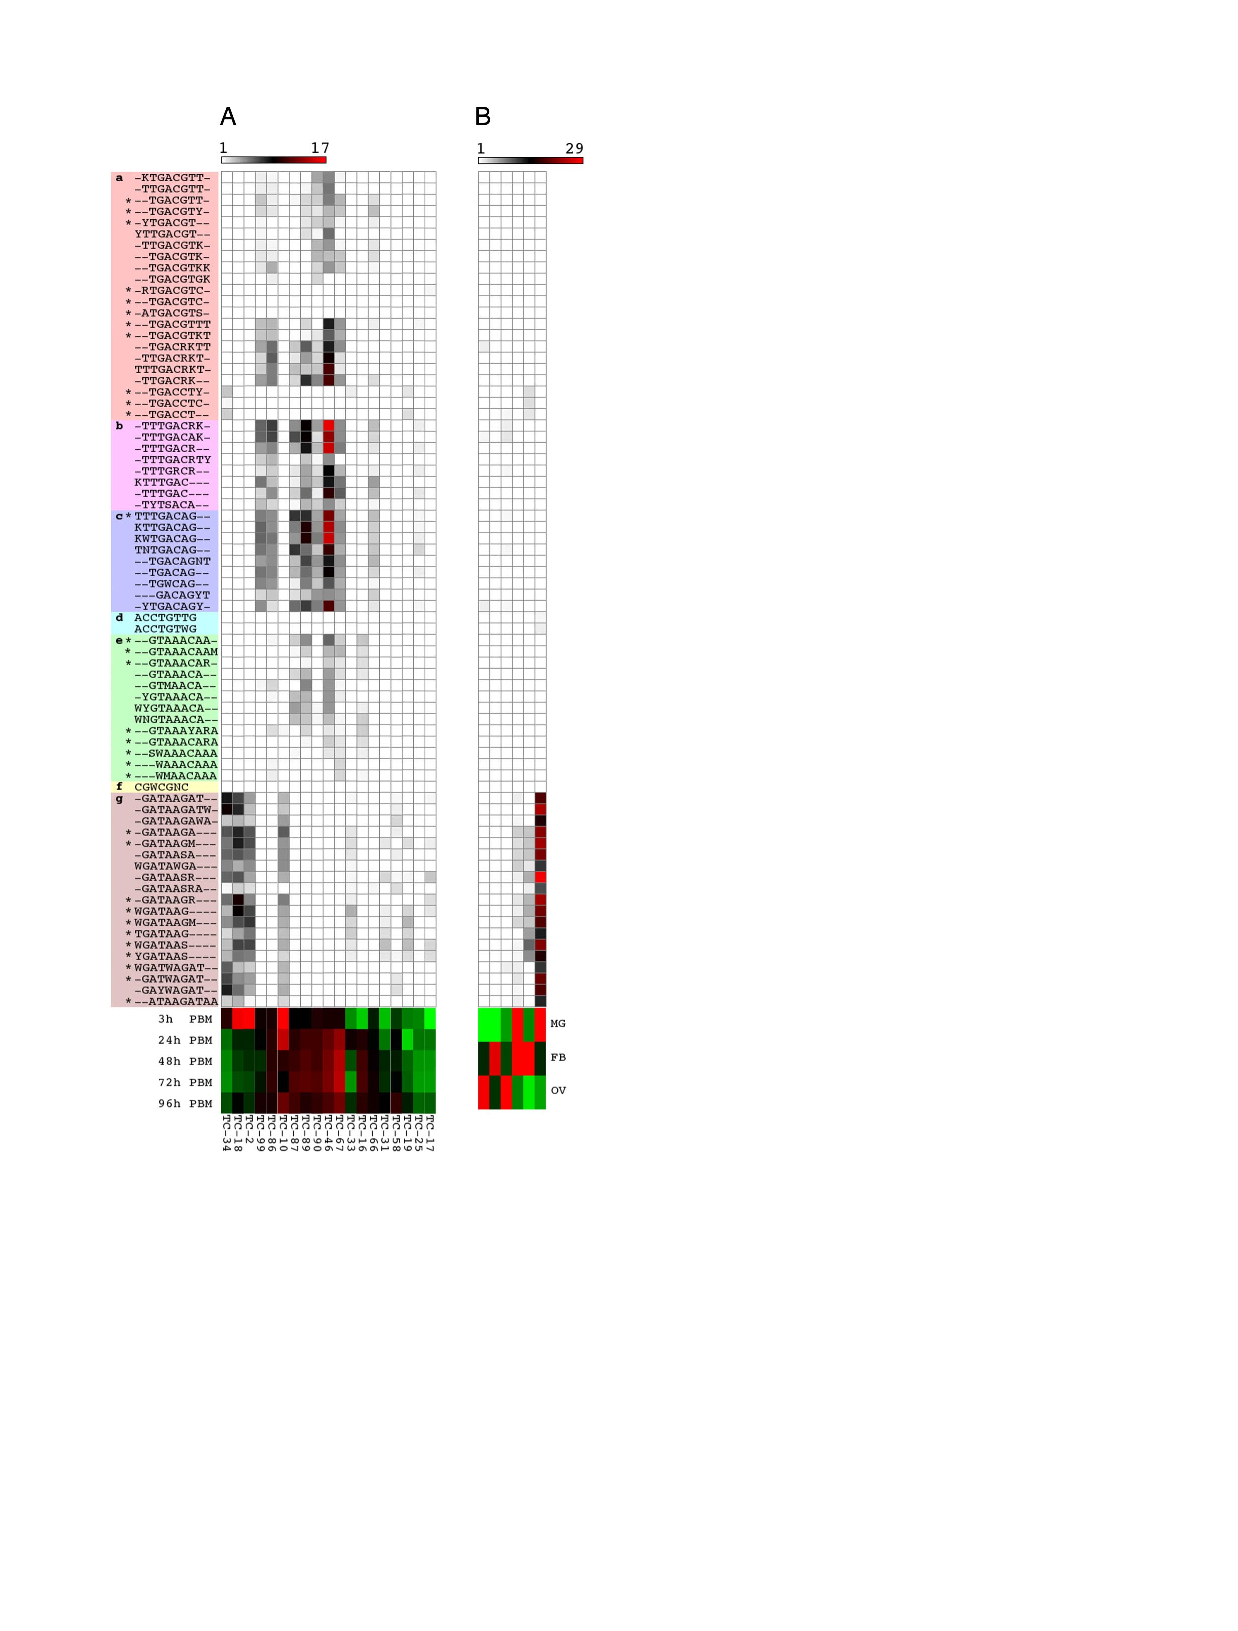
\includegraphics[scale=.95]{figures/figs/sieglaff2009_full.pdf}
\hfil
\caption[Associations of mosquito motifs with gene expression profiles in \Ag]{\bsf{Associations of mosquito motifs with gene expression profiles in \Ag:} \\ \sf
Motif enrichment within (A) 5′-end flanking regions of genes in clusters responsive to blood meal ingestion, and in (B) 5′-end flanking regions of genes in clusters enriched in selected tissues. The significance of motif enrichment is indicated by pseudocolor of -log10 (P-value) determined through hypergeometric statistics, and the median expression profile of each gene cluster is shown below each respective column. Red and green colors represent higher and lower relative mRNA accumulation, respectively. Asterisks (*) indicate a match to a previously described mosquito TFBS. Heatmaps were created with Matrix2png (\CITEME:local-58). FB, fat body; hPBM, hours post blood meal; MG, midgut; OV, ovaries; TC, time course clusters.

Adapted from \cite{Sieglaff2009}}
\label{fig:sieglaff2009_full}
\end{figure}

% [*\CITEME 3]  \cite{Nene2007}
% [*\CITEME 10] \cite{Wu2008}
% [*\CITEME 25] \cite{Kokoza2001}
% [*\CITEME 26] \cite{Cho2006}
% [*\CITEME 28] \cite{Attardo2003}
% [*\CITEME 29] \cite{Ahmed1999}
% [*\CITEME 30] \cite{Pham2005}
% [*\CITEME 32] \cite{Giannoni2001}
% [*\CITEME 33] \cite{Davidson2010}
% [*\CITEME 34] \cite{Das2007a}
% [*\CITEME 35] \cite{Hu2005}
% [*\CITEME 36] \cite{Tompa2005}
% [*\CITEME 37] \cite{Wasserman2004}
% [*\CITEME 38] \cite{Elemento2005}
% [*\CITEME 39] \cite{Stark2007}
% [*\CITEME 40] \cite{Xie2005}
% [*\CITEME 41] \cite{Dittmer2003}
% [*\CITEME 42] \cite{Meredith2006}
% [*\CITEME 43] \cite{Hernandez-Romano2008}
% [*\CITEME 44] \cite{Rai1999a}
% [*\CITEME 45] \cite{Borkent2004}
% [*\CITEME 46] \cite{Calvo2006}
% [*\CITEME 47] \cite{Adelman2007}
% [*\CITEME 48] \cite{Xu2005a}
% [*\CITEME 49] \cite{Jasinskiene2007}



The role \glspl{CRE} play in regulating gene expression during development is well-established \cite{Davidson2010}, and the development of tools for their identification is an active area of research following the publication of genome sequence and associated genome-wide expression datasets. However, the discovery \textit{in silico} of \glspl{CRE} is challenging because typically they are short, degenerate, and contained within vast amounts of intergenic genomic DNA. Despite these limitations, various computational approaches have been developed for their discovery \cite{Das2007a,Hu2005,Tompa2005,Wasserman2004}. Comparative genomics represents a powerful extension to \gls{CRE} discovery that diminishes these effects. Functional gene regulatory elements, including \glspl{CRE}, are proposed to diverge at much lower rates compared to neutral sequences because of selective pressures, and therefore may stand out from surrounding neutral DNA by virtue of their greater levels of conservation among orthologous sequences. Previous work has demonstrated the utility of this concept \cite{Elemento2005,Stark2007,Xie2005} and comparative genomics of insects has been applied successfully to map putative \glspl{CRE} in the genomes of relatively closely related \textit{Drosophila} species, [divergence times estimated ≤ 50 \gls{Mya} \cite{Stark2007} (Figure \ref{fig:mosqPhyloTree})], in which orthologous intergenic sequences are aligned more easily. The work represented by \citet{Sieglaff2009} includes mosquito species with phylogenetic relationships spanning 20 to 200 \gls{Mya} with genomic comparisons complicated by large amounts of dispersed repetitive elements \cite{Nene2007}.

The \gls{MDOS} algorithm \cite{Wu2008} was designed to mitigate these problems by not requiring alignment of orthologous sequences, and incorporating features that account for the greater probability for the co-occurrence of a motif because of shared ancestry in orthologous sequences. The application of \gls{MDOS} for computational discovery of putative \glspl{CRE} shared among mosquitoes resulted in the identification of mosquito-specific or enriched motifs. These motifs demonstrate that \gls{MDOS} can identify related DNA sequences in diverged mosquitoes and may be useful in similar scenarios in which genome sequences are being analyzed for species that have no other closely related genomes available. Furthermore, the identification \textit{in silico} of GATA-factor and other \glspl{TFBS} that are identical to those whose function was established experimentally \cite{Kokoza2001,Cho2006,Attardo2003,Ahmed1999,Pham2005,Giannoni2001,Dittmer2003,Meredith2006} serves as a powerful positive control for these analyses. The 5′-end regions of immune-related genes from \Ag\ and \Dm\ were screened for conserved motifs, and AT-rich domains were found to associate with \gls{NFKB} response elements \cite{Hernandez-Romano2008}. These sequences were not identified in these analyses because the restrictions on the dataset used eliminated many of the immune-related genes where one-to-one orthology may be difficult to establish. In addition, most AT-rich domains discovered in their study were ≤ 6 nucleotides in length, and these analyses only addressed those recovered with lengths of 7 to 9 nucleotides.

The 3 mosquito species included in \citet{Sieglaff2009} require a bloodmeal for successful reproduction. Although this trait is not unique to this group of arthropods, acquiring the necessary nutrients for egg development from ingested blood is a specialized adaptation in insects. There is debate on when and how \gls{hematophagy} arose in mosquito evolution \cite{Rai1999a}, but it is hypothesized that the occurrence of this trait in the larger clade is \gls{monophyletic} \cite{Borkent2004,Calvo2006}. Most of the discovered mosquito motifs are associated with bloodmeal-regulated genes. Thus, these data support a common hematophagous ancestor for all mosquitoes, and indicate that \gls{hematophagy} acts as a selective force for conservation of \glspl{CRE}.

The functionality of some of the discovered motifs was supported further in \Ag\ and \Aa\ by their association with genes displaying enriched transcription product accumulation within tissues responsible for bloodmeal digestion and reproduction (Figure \ref{fig:sieglaff2009_full}). These findings bolster the conclusion that these mosquitoes share a regulatory code controlling expression levels for some genes regulated after \gls{hematophagy}. The availability of additional genome-wide studies of gene expression for all 3 mosquito species will facilitate discovery of other associations of the motifs with specific gene-regulation patterns.

\citet{Sieglaff2009} and similar genome-wide approaches to identify putative \glspl{CRE} in mosquitoes \cite{Hernandez-Romano2008} are furthering our understanding of the mechanisms involved in gene regulation in this group of vector insects. An expanded set of putative mosquito \glspl{CRE} will allow the definition of genome-wide motif-association maps and the identification of \glspl{CRM} comprising multiple, linked \glspl{CRE} that convey specific patterns of gene expression. Experimental validation of the functionality of each discovered motif and regulatory module is necessary and will provide support for the development of mosquito synthetic promoters that deliver desired and predetermined expression patterns in transgenic mosquitoes. 
The availability of defined synthetic mosquito promoters that direct controlled, local gene expression in response to pathogens also would be a major advance. These promoters would allow engineering of mosquitoes with increased parasite or virus resistance. These and similar envisioned applications for mosquito control and the control of mosquito-borne disease transmission will benefit greatly from a better understanding of gene regulation mechanisms in these insects.










\pagebreak

\section{RNA-seq analyses of blood-induced changes in gene expression in the mosquito vector species, \Aea\ \cite{Bonizzoni2011}}
% [-17] Brackney2010
% [-31] Fischer2008
% [-32] Pane2007
% [-33] Lawson2009
% [-50] Salazar2007
% [-54] Marelli2006
% [-55] Amenya2010
% [-56] Carlson2007
% [-57] Kriventseva2008
% [-58] Sieglaff2009
% [-60] Hubbard2002
% [-61] GENEBUILD?
% [-62] Bennet2002
% [-63] Black2002
% [-64] Terenius2008



Bonizzoni and Dunn \cite{Bonizzoni2011} provides a detailed examination of the changes in transcripts accumulation occurring at the whole-body level of \Aa\  females 5 hours \gls{PBM}. The observed changes are consistent with the beginning of an intense physiological response to a bloodmeal. The majority of immunity-related transcripts tended to accumulate at lower levels in bloodfed mosquitoes. This finding supports the hypothesis that there may be a gap in immunity following a bloodmeal. Reduced expression of immune genes in bloodfed mosquitoes could favor the establishment of infections, especially considering that pathogens such as dengue viruses infect the midgut epithelial cells within minutes after the contact \cite{Salazar2007}. However, changes in transcript abundance observed at the whole-body level may mask changes in accumulation occurring primarily in the midgut. Different levels of activation of immunity genes after a blood feeding may be one of the factors contributing to the variability in vector competence for dengue viruses observed in different geographic populations of \Aa\  \cite{Bennett2002},\cite{Black2002}. The quantity and quality of data generated by RNA-seq technology makes it an ideal approach for comparative analyses of the transcriptome of \Aa\ strains with different vector competence and vectorial capacity.

Our analyses of the expression profiles of sugarfed (S) and bloodfed (B) mosquitoes allowed the identification of co-regulated genes and putative \textit{cis}-regulatory elements and modules from the \Aa\  genome. Further knowledge of the mechanisms involved in regulation of gene expression in vector species is critical to the development of control strategies whereby the vector is modified genetically to express anti-pathogen effector molecules in tissue-specific and time-regulated manners \cite{Terenius2008}. Promoter and other \textit{cis}-acting regulatory DNA fragments are needed to regulate restricted expression of selected anti-pathogen effector molecules. Moreover, we described several examples of how the RNA-seq data generated can help improve the current annotation of the \Aa\  genome.

\subsection{Transcripts found exclusively in bloodfed mosquitoes}
Forty transcripts were found only in bloodfed mosquitoes, with the highest read-counts reaching ~1000/transcript, after normalizing for different library sizes (data not shown). Functional parent attribution for these transcripts is consistent with a role in digestion and in the progression of the gonotrophic cycle. Specifically, two transcripts, Aa5G1 (AAE013712-RA) and AaSPVI (AAE010196-RA), correspond to the midgut serine proteases shown previously to be elicited by a bloodmeal in the midgut of \Aa\  females \cite{Brackney2010}. Seven other transcripts encode enzymes (i.e. decarboxylase, cathepsin b and trypsins), and two are implicated in trafficking. Transcripts AAE014815-RA and AAE005950-RB correspond to the vacuolar protein sorting 13B from yeast and the chloride channel protein 2, respectively. Ten transcripts are orthologous to the G12 gene of \Ag\ and share the Insect Allergen Repeat motif. This motif is hypothesized to be a novel, insect-specific detoxifying domain implicated in the co-evolution of herbivorous insects and their plant hosts and also has been linked to nitrile-specific detoxification \cite{Fischer2008}. Transcripts AAEL006126-RB and AAEL008921-RC are predicted orthologues of the \Cxq\ vitellogenin-A1 gene and the \Dmel\ spaghetti squash (sqh) gene, respectively. The sqh gene product encodes the regulatory light-chain of non-muscle myosin II, which is required for cytoplasmic transport in nurse cells during oogenesis and also has been implicated in germline \gls{RNAi} processes \cite{Pane2007}.

\subsection{\textit{Cis}-regulatory element discovery}
Tightly regulated and bloodmeal-induced expression profiles are of particular interest for designing transgenic mosquito-based control strategies to reduce transmission of dengue fever. \textit{Cis}-regulatory sequences derived from bloodmeal-induced / up-regulated mosquito genes allow potentiating swift induction and effective levels of transcription of an associated effector gene, while likely inflicting the least fitness cost \cite{Marelli2006}, \cite{Amenya2010}. We interpret the different levels of mRNA accumulation seen in this study to reflect changes in transcriptional activity of the corresponding genes, although it is possible that some levels may vary as a function of changing transcript stability or rates of turnover. With this in mind, we used \gls{SCOPE} \cite{Carlson2007} to predict putative \glspl{CRE} that may provide the basis for rational identification and selection of new candidate promoter regions and for modification of the transcriptional profiles of current transgene constructs. We examined the 2000 base pairs (bp) flanking the 5'-boundaries of the 40 transcripts that were undetected in libraries from sugarfed mosquitoes but detected at significant levels in the RNA-seq libraries from bloodfed mosquitoes and identified a redundant list of 22 motifs that are enriched significantly in these sequences (Figure \ref{fig:bonizzoni2011-cres}). A possible \gls{CRM} constructed with the discovered \glspl{CRE} is represented by the motif consensus sequences, \texttt{cnatcnkcwgtt}, \texttt{gyactyvar}, and \texttt{tgakamga}, and is associated with \Aa\  orthologs of the G12 gene of \Ag\ (AGAP006187) (Figure \ref{fig:bonizzoni2011-cres}). \Aa\ has 17 G12 genes, many more relative to other insects, which have 4.5 on average (according to OrthoDB; group EOG95TCTG) \cite{Kriventseva2008}. The transcripts of nine of the G12 orthologs are present in this co-regulated gene set (representing ~25\% of the 40).

Another putative \gls{CRM} contains the consensus sequence \texttt{tgakamga}, \texttt{cnatcnkcwgtt}, \texttt{asttrccc} and \texttt{aarcttbd} (Figure \ref{fig:bonizzoni2011-cres}). This \gls{CRM} groups with the cathepsin b genes, AAEL015312-RA and AAEL007585-RA. Verification of these \glspl{CRM} will require empirical testing, however, the top 10 matches for \texttt{tgakamga}, which is present in both putative \glspl{CRM}, align well to members of the mosquito-conserved GATA motifs correlated to transcriptional responses to blood feeding in \Ag\ \cite{Sieglaff2009}.





\subsection{RNA-seq identifies annotation corrections}


\begin{figure}[hp]
\centering
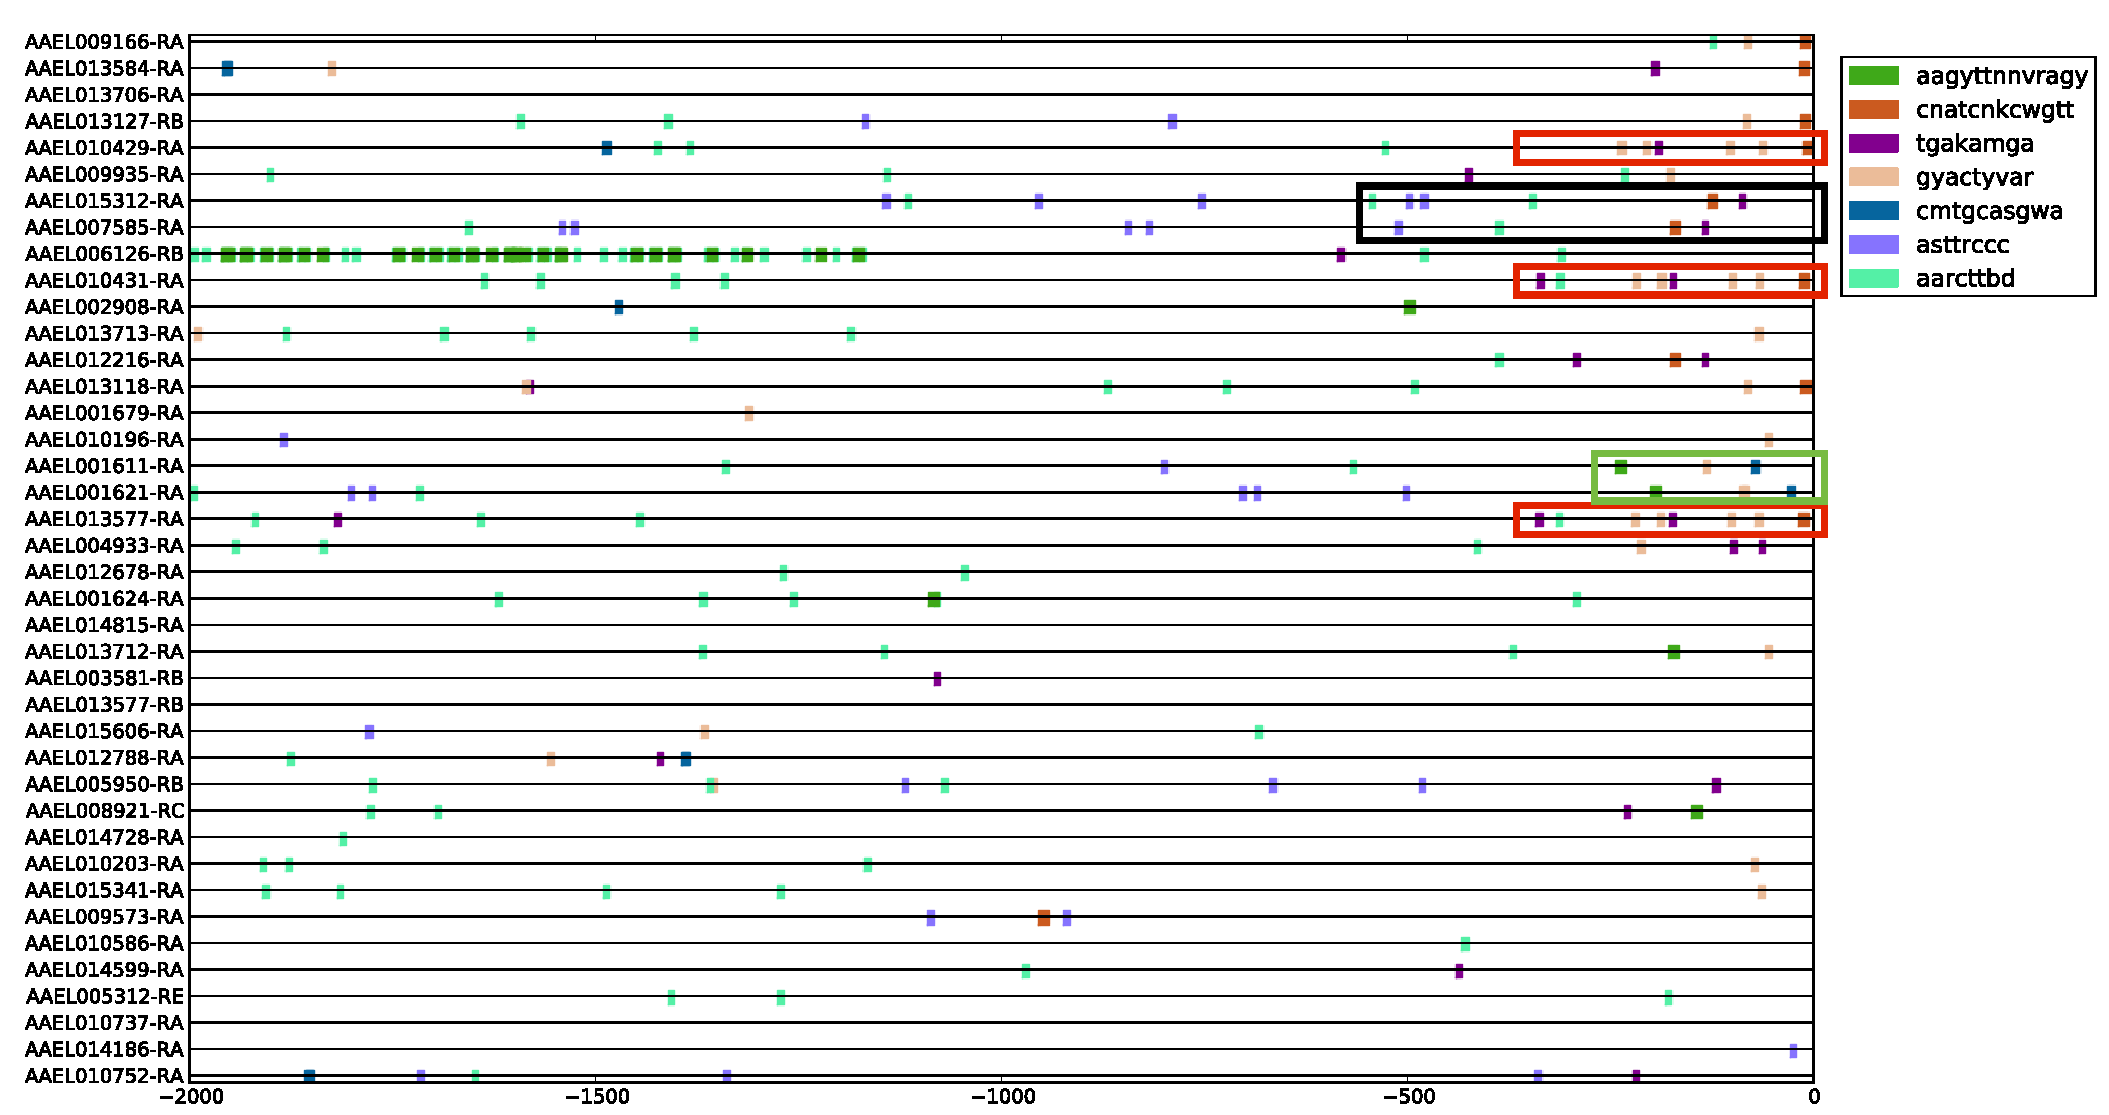
\includegraphics[width=.99\textwidth]{figures/figs/bonizzoni2011-cres.pdf}

\caption[Motif map of putative CREs from transcripts detected only in bloodfed female \Aa]{\sf \textbf{Motif map of putative CREs discovered by SCOPE using transcripts detected significantly only in bloodfed female \Aa:} Locations of representative SCOPE-derived CRE motifs in the 2000 bp upstream of the annotated translational start site in the 40 transcripts detected significantly only in bloodfed females. Transcript names on the left are ordered from most (top) to least (bottom) abundant.  Candidate CRMs are highlighted in like-colored rectangles.

Adapted from \cite{Bonizzoni2011}}
\label{fig:bonizzoni2011-cres}
\end{figure}

\begin{figure}[hp]
\centering
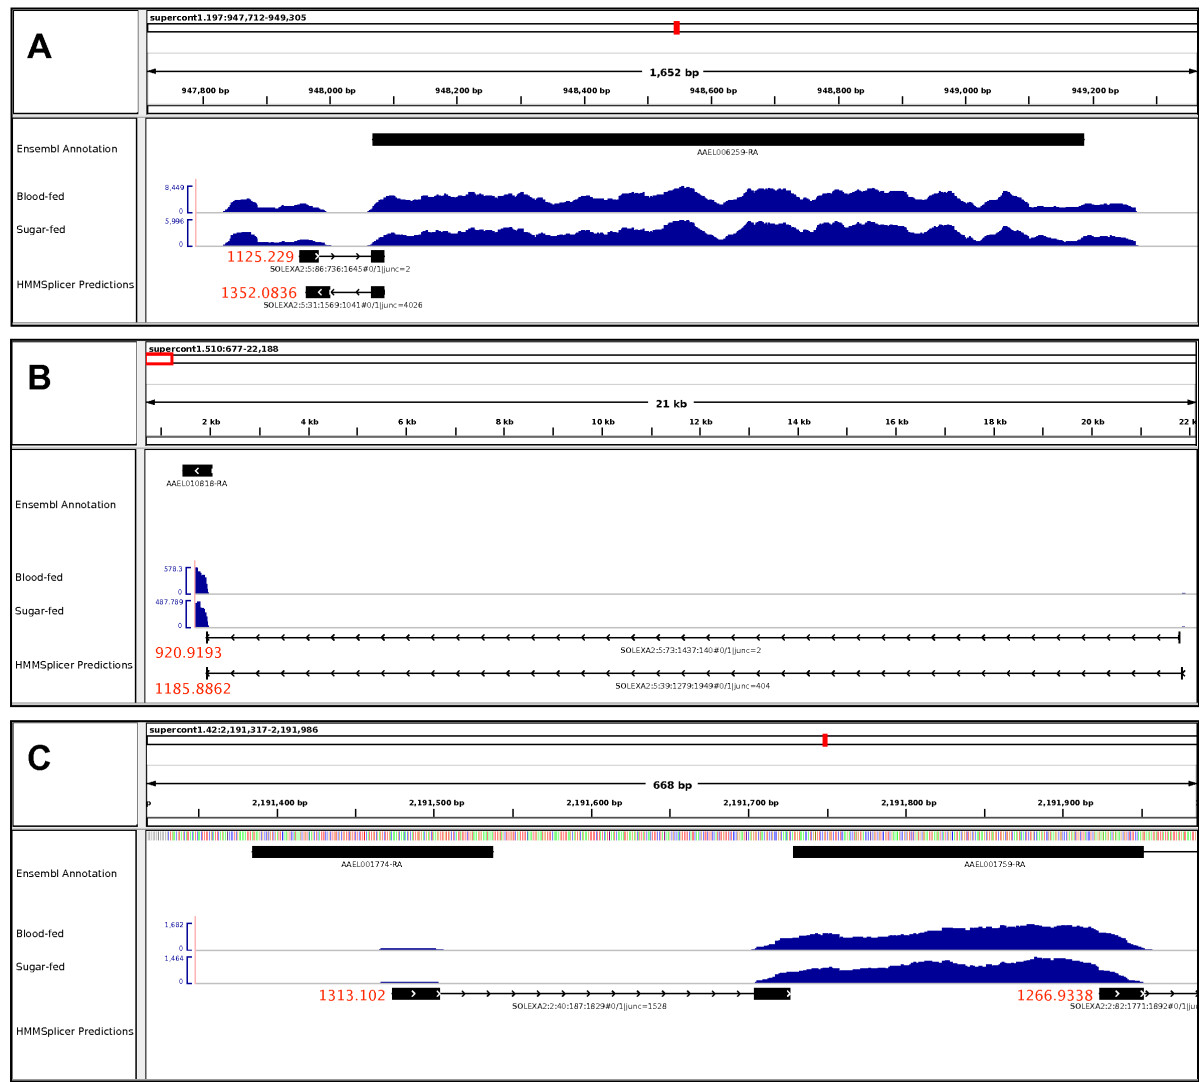
\includegraphics[width=.95\textwidth]{figures/figs/aedesHMMsplice.jpg}

\caption[Examples of amendments to the \Aa\ annotation supported by HMMSplicer results]{\sf \textbf{Examples of amendments to the \Aa\ annotation supported by HMMSplicer results:} Black bars in the top tracks represent the current gene annotations. Blue histograms in the second track represent the non-normalized coverage of RNA-seq reads at each position. The range of the histogram values shown in each view is depicted on the labeled y-axis of each RNA-seq track. Black boxes in the lower track represent splice-site predictions based on the RNA-seq reads using HMMSplicer determined in this study. Each function has a unique identifier listed below and its HMMSplicer score is listed in red. If multiple reads support a single junction, "junc = x" lists the number of supporting reads. This information provides evidence to link two islands of transcription as a single transcription event, therefore, exons of a common mRNA. All predicted junctions shown here also are supported by EST alignments. Genes are (A) AAEL006259; (B) AAEL010818; and (C) AAEL001774 and AAEL001759.

Excerpted from \cite{Bonizzoni2011}}
\label{fig:aedesHMMsplice}
\end{figure}
\begin{table}[hp]
 \begin{center} \sf
\begin{tabular}{cc}\toprule
\textbf{Distance from annotation (bp)} & \textbf{Predicted junctions}\\ \midrule
0-1000 & 1170\\
1001-2000 & 120\\
2001-4000 & 149\\
4001-8000 & 245\\
8001-16000 & 486\\
16001-32000 & 517\\
> 32000 & 854\\ \midrule
\textbf{Total} & \textbf{3541}\\ \bottomrule
 \end{tabular}
 \end{center}

\caption[Predicted novel junctions within various symmetric distance-windows from annotated transcripts]{\sf \textbf{Predicted novel junctions within various symmetric distance-windows from annotated transcripts:} \\
(Gene build AaegL1.2)\\
Excerpted from \cite{Bonizzoni2011}}

\label{tab:bonizzoni2011-novel-junx}
\end{table} 

RNA-seq also provides an opportunity to examine and improve the current annotation of the \Aa\  genome and examine the level of transcriptome plasticity in terms of alternative splicing. We used HMMSplicer \cite{Dimon2010} to compare junctions revealed by our data to the annotation provided by Vectorbase and Ensembl \cite{Lawson2009,Hubbard2002}. HMMSplicer predicted 32,501 junctions supported by at least two RNA-seq reads using the combined data from sugar and bloodfed samples. Of these, 24,100 (74\%) matched junctions present in the AaegL1.2 gene-build provided by VectorBase, leaving 8,401 predicted novel high-scoring splice sites supported by multiple RNA-seq reads. A total of 4500 (~54\%) of these occur within annotated gene boundaries and may represent un-annotated alternatively-spliced transcripts. To estimate how many of the remaining splice junctions might be truly novel, we mapped them to increasingly larger DNA fragments flanking the currently-annotated genes (Table \ref{tab:bonizzoni2011-novel-junx}). A total of 2687 (~33\%) junctions mapped within 32,000 bp of the 5'- or 3'-ends of annotated gene boundaries. Of these, 1439 mapped within 4000 bp, consistent with the interpretation that they may represent alternatively-spliced transcripts of the previously-identified genes. Those mapping beyond 4000 bp could be alternate junctions of the known genes, represent un-annotated transcription products, or be artifacts.


An accurate gene annotation, especially with respect to the \gls{TSS}, is considerably advantageous with respect to the accurate discovery of \glspl{CRE} because prediction tools must make the assumption that the sequences included are true regulatory regions, and their performance suffers when this is false. For the \gls{CRE} predictions described in the previous section, 36 of the 40 transcript start sites were in close agreement to the Ensembl annotation \cite{Hubbard2002}. Figure \ref{fig:aedesHMMsplice} highlights three determined amendments to the current annotation, all supported by EST data. Figure \ref{fig:aedesHMMsplice} (A and B) supports the conclusion that the current annotation has missed the putative first exons that extend the 5'-UTRs of some genes (AAEL006259, AAEL010818) and provides additional information for predicting accurate \glspl{TSS}. In the case of AAEL010818, the \gls{TSS} determined by RNA-seq data is 20 kb to the 5'-end of the annotated start site, far outside the distances commonly searched for \glspl{CRE} (Figure \ref{fig:aedesHMMsplice} B). In some cases, as was seen for AAEL001774, the first exon was annotated but included as a separate gene model, which also contains the likely 5'-UTR of AAEL001759 (Figure \ref{fig:aedesHMMsplice} C). AAEL001774 encodes a protein comprising 50 amino acids with no known functional domains aside from a predicted signal peptide that makes up 66\% of its length.










\pagebreak
\section{Complex modulation of the \Aea\ transcriptome in response to dengue virus infection. \cite{bonizzoni2012complex}}
%\todo[inline]{import text for COMPLEX MODULATION OF AEDES TXOME}


The World Health Organization lists dengue as the most important arthropod-borne viral disease of humans \cite{WHO2009}.
The major vector of all four dengue virus serotypes (\gls{DENV}1–4) is the cosmopolitan mosquito, \Aea.
Close association with human populations and increasing intercontinental travel favor the expansion of its geographic distribution.
There are no effective prophylactic and therapeutic drugs specific for dengue, and vaccine development is hindered by potential antibody-dependent enhancement that could put people at greater risk of life-threatening, severe dengue \cite{Gubler2002}.
As a consequence, vector control is currently the only practical and effective strategy for disease prevention.
The \Aa\ genome was sequenced and knowledge of genome-wide changes in patterns of gene expression following \gls{DENV} infection is expected to identify genes involved in vector competence, the intrinsic ability of the mosquito to host and transmit \gls{DENV} \cite{Nene2007}, \cite{Kramer2003}.
This knowledge, coupled with germline transformation technology and anti-viral effector molecules, can be applied to the development of genetically-modified mosquitoes incapable of arbovirus transmission \cite{James2007}, \cite{Franz2006}, \cite{Mathur2010}.

Although vertical transmission of dengue viruses has been reported, mosquitoes become infected mainly following ingestion of an infectious-bloodmeal \cite{Gunther2007}, \cite{Angel2008}.
Viruses are transmitted to new human hosts during a subsequent bloodmeal following an \gls{EIP} of 7–14 days.
The duration of the \gls{EIP} depends on the mosquito strain, virus genotype and environmental factors \cite{Watts1987}, \cite{Black2002}, \cite{Anderson2006}, \cite{Salazar2007}, \cite{Lambrechts2011}.
During the first 1–2 \gls{dpi}, \gls{DENV}s invade midgut epithelial cells through receptor-mediated endocytosis and initiate replication \cite{Bennett2002}, \cite{Heinz2003}, \cite{Rey2003}, \cite{Mercado-Curiel2008}.
These processes involve both viral and host cellular factors \cite{Samsa2009}.
Infection spreads laterally in the midgut epithelium to cells adjacent to those infected originally \cite{Salazar2007}.
Virus titers peak in the midgut usually between 7–10 \gls{dpi} and are followed by a decline \cite{Salazar2007}, \cite{Xi2008}.
\gls{DENV} infection disseminates from the midgut throughout the body, presumably through the tracheal system, reaching the salivary glands as early as 3 \gls{dpi} \cite{Salazar2007}.
Maximum virus titers in the salivary glands are reached 12–18 \gls{dpi}.
The saliva of an infected mosquito containing \gls{DENV}s is injected in a human host during feeding to complete the transmission cycle.

\Aea\ populations of different geographic origin vary in their vector competence.
Phenotypes include those in which \gls{DENV}s either cannot establish a midgut infection (Midgut Infection Barrier) or cannot disseminate to other tissues (Midgut Escape Barrier) \cite{Black2002}, \cite{Gubler1976}, \cite{Cox2011}.
Other phenotypes manifest in the absence of virions in the saliva (Transmission Barrier).
Differences in intensity of infection (peak titers) and duration of \gls{EIP} also are observed among mosquito strains \cite{Salazar2007}.

Multiple quantitative trait loci are associated with MIB and MEB, but specific genes have yet to be identified \cite{Black2002}.
Mosquito genes and physiological pathways related to innate immunity, redox activity, energy production and metabolism are modulated in response to \gls{DENV} infection \cite{Xi2008}, \cite{Sanchez-Vargas2009}, \cite{Sim2010}, \cite{Tchankouo-Nguetcheu2010}, \cite{Luplertlop2011}, \cite{Behura2011}, \cite{Sim2012}, \cite{Colpitts2011}.
These observations come from multiple studies of specific mosquito tissues and time points following infection, and used different combinations of \gls{DENV}2 genotypes and \Aa\ strains.

We investigated genome-wide changes in transcript accumulation in mosquito midguts, carcasses and salivary glands at 1, 4 and 14 \gls{dpi} during the course of \gls{DENV}2 infection.
This analysis was conducted by RNA-seq with the Chetumal (CTM) strain of \Aa\ and \gls{DENV}2-Jam1409.
\gls{CTM} was colonized recently (2005) from mosquitoes from the Yucatan Peninsula and is well-characterized for its response to non-infectious bloodmeals and for the kinetics of \gls{DENV}2-Jam1409 infection \cite{Salazar2007}, \cite{Bernhardt2012}, \cite{bonizzoni2012strain}.
A total of 397 genes had transcripts that showed statistically-significant differential accumulation following \gls{DENV} infection, comprising both those found previously and those that are novel to this study, emphasizing the complex interaction between \Aa\ and \gls{DENV}s \cite{Xi2008}, \cite{Sim2010}, \cite{Tchankouo-Nguetcheu2010}, \cite{Luplertlop2011}, \cite{Behura2011}, \cite{Sim2012}, \cite{Colpitts2011}.




\subsection{Results}
\subsubsection{RNA Sequencing and Mapping Summary}

Illumina RNA-seq technology was applied to study the accumulation levels of poly-adenylated RNAs at 1, 4 and 14 \gls{dpi} in the carcasses and corresponding midguts of \gls{CTM} females fed either a non-infectious (B) or \gls{DENV}2-infected (\gls{DENVI}) bloodmeal.
Accumulation levels also were assessed in the salivary glands at 14 \gls{dpi}.
Single-end RNA-seq libraries were constructed starting from pools of 20–40 mosquitoes.
Each RNA-seq library generated between 14 and 45 million 40 bp reads (not shown).
Sequenced reads were mapped by TopHat \cite{Trapnell2009} to the \Aa\ transcriptome.
The accumulation levels of specific poly-adenylated RNAs were compared between B and \gls{DENVI} samples at each time point/conditions using DESeq \cite{Anders2010} and Cufflinks \cite{Trapnell2010} (not shown).
Genes whose products were identified as significantly differentially accumulated by DESeq are contained mostly within the larger number designated similarly by Cufflinks (not shown). A total of 397 unique genes have poly-adenylated RNAs identified by both DESseq and Cufflinks as accumulated differentially and significantly between B and \gls{DENVI} mosquitoes

\subsubsection{Discovery of cis-regulatory Elements}

Genes with similar expression profiles may share common regulatory mechanisms, including the occurrence of similar \glspl{CRE} \cite{Sieglaff2009}.
Evidence of this shared regulation may be evident in the control DNA sequences of mosquito genes that are expressed exclusively or highly-induced following dengue virus infection.
Some of these genes also may have transcripts that accumulate to high or higher levels following an uninfected bloodmeal (B samples).
The preferred expression profile for an antiviral effector gene would be one that is induced highly after blood feeding and is either further elevated or not affected by virus infection.

A total of 2012 genes showed read-coverage in salivary glands of \gls{DENVI} mosquitoes but not in the salivary glands of B mosquitoes.
While fifteen of these genes were associated with lipid metabolism, the majority were related to transcription and translation and/or chromatin structure and dynamics (not shown).
Forty-one of these had FPKM$_{DENVI}$ ≥ 15, and only one, AAEL005034, showed tissue-specific expression (not shown).
As many as 762 and 1324 genes had transcripts that were detected in infected but not in the corresponding uninfected carcasses and midguts samples, respectively.
The vast majority of these had FPKM$_{DENVI}$ < 4.
The exceptions were AAEL011066, AAEL010034 and AAEL002899, all encoding hypothetical proteins.
At 1\gls{dpi}, AAEL011066 had read coverage only in carcass of \gls{DENVI} (FPKM$_{DENVI}$ = 14.97); AAEL010034 and AAEL002899 in midguts of \gls{DENVI} (FPKM$_{DENVI}$ = 8.11 and 6.56, respectively) (not shown).
The putative promoter regions of 41 genes with FPKM$_{DENVI}$ ≥ 15 in salivary glands were analyzed using MEME \cite{Bailey2006} (Figure \ref{fig:bon2012complex-S2}).

We refined the search for common, co-occurring \glspl{CRE} by considering the promoters of genes whose products accumulated highly (FPKM$_{DENVI}$ ≥ 100) in \gls{DENVI} mosquitoes and were at the same or lower levels (FPKM$_{B}$ ≤ 100) in B mosquitoes (not shown).
The latter criterion eliminates all genes whose accumulation levels are lowered in the presence of a dengue infection.
In addition, this grouping also contains genes whose transcripts do not have a significant differential accumulation between infected and uninfected mosquitoes.
The results support the presence of a module composed of six motifs (Figure \ref{fig:bon2012complex-S3}: motifs 2, 4, 5, 6, 8, 10) in 4/51 genes with FPKM$_{DENVI}$ > 100 in midguts at 1 and 4 \gls{dpi}.
The four genes sharing this module (AAEL007162 [APG8], AAEL001593 [glycerol-3-phosphate dehydrogenase (G3PDH)], AAEL003046 [saponin], AAEL000291 [V-type proton ATPase 16 kD proteolipid subunit (V-ATPase)]) had transcripts that were more abundant (1.03–1.64 fold) in \gls{DENVI} than B mosquitoes in midguts samples at 1 and 4 \gls{dpi}.
These genes are not related functionally, but are associated with lipid metabolism, which has been shown to play an important role during \gls{DENV} life cycle \cite{Samsa2009}.
Furthermore, G3PDH links carbohydrate and lipid metabolism.
The V-ATPase may be required to maintain transmembrane charge differential for virus entry.
Saponin is a regulator of lipid degrading enzymes \cite{Lindholm2010}.
These genes, with the exception of that encoding G3PDH, had transcripts with FPKM$_{DENVI}$ > 100 also in carcasses and salivary glands, but were not consistently higher or equally-abundant in \gls{DENVI} than B mosquitoes.
Transcripts encoding the V-ATPase were more abundant in \gls{DENVI} mosquitoes of the susceptible MOYO-S strain three hours post infection (hpi) with \gls{DENV}2 Jam1409 \cite{Behura2011}.
Matches to transcription factors in the TRASFAC- database \cite{Matys2006} and supported by an e-value ≤ $10^{-5}$ were identified for motifs 4, 5, 6 and 10.
The highest match of Motif 4 is Blimp1, which is an ecdysone-inducible transcription factor involved in Drosophila development, metamorphosis and oogenesis \cite{Agawa2007}.
Motif 5 matched highest with Rel.
The Rel or \gls{NFKB} superfamily of conserved eukaryotic proteins is involved in the control of immune and inflammatory responses, developmental processes, cellular growth and apoptosis.
Motif 6 has high matches with High Mobility Group (HMG), Broad-Complex (BRC) and Forkhead transcription factors.
HMG transcription factors are implicated in replication, recombination and DNA repair \cite{Rajeswari2002}.
BRC is an ecdysone-regulated transcription factor implicated in developmental processes in \Dm\ \cite{Sandstrom1997}.
The Forkhead family of transcription factors includes seventeen sub-classes regulating development, homeostasis and reproduction in insects \cite{Hansen2007}.
Motif 10 matches best with the NK-2-Nkx\_TTF1 transcription factor, a homeodomain-containing transcription factor implicated in morphogenesis, differentiation and tissue-specific maintenance \cite{Boggaram2009}.

MEME analyses on the putative promoter regions of the 83 genes that had FPKM$_{DENVI}$ ≥ 100 in carcasses consistently from 1 to 14 \gls{dpi} showed the presence of three to five motifs (Figure \ref{fig:bon2012complex-S4}: motifs 1, 2, 5, 7, 8) grouped tightly in eight genes (AAEL010097 [hypothetical protein], AAEL012629 [deoxyuridine 5′-triphosphate nucleotidohydrolase], AAEL008041 [bleomycin hydrolase], AAEL013068 [protein phsophatase-2a], AAEL017269 [novel protein coding], AAEL009604 [hypothetical protein], AAEL003552 [DNA-directed RNA polymerase subunit rpb6] and AAEL000739 [hypothetical protein]).
Different combinations of these motifs are found in seven additional genes: (AAEL008849 [selenophosphate synthase], AAEL014903 [40S ribosomal protein S24], AAEL004484 [predicted protein], AAEL008768 [multiprotein bridging factor], AAEL009274 [hypothetical protein], AAEL001061 [glutathione transferase], AAEL012279 [eIF3j] and AAEL009320 [chaperonin]).
This motif group is designated provisionally the “carcass module”.
All 15 of these genes also had read coverage in midguts and salivary glands, but the abundance of the corresponding transcripts was not always as high (FPKM$_{DENVI}$ = ≤100), and in some cases they are more abundant in B than \gls{DENVI} mosquitoes.
AAEL017269 and AAEL000739 had read coverage only in salivary gland samples of \gls{DENVI} mosquitoes.

Motif 1 could be the binding site for the transcription factor MADS\_MCM1+SFF\_M01051 (e-value = $7.36E-06$).
The MADS-box family of transcription factors is conserved among yeasts, plants, insects, amphibians and mammals.
It includes proteins associated with different biological roles (pheromone response, muscle-specific gene regulation, development) that operate generally by specifically recruiting other transcription factors into multi-component regulatory complexes \cite{Shore1995}.
Motif 2 has its best match to bZIP-type transcription factors (e-value = $2.27E-06$).
bZIP proteins belong to the largest and most conserved superfamily of transcription factors, the basic region leucine zipper transcription factors, involved in regulation of development, metabolism, and other cell functions such as secretion, oxidative stress and response to pathogens \cite{Miller2009}, \cite{Abrams2005}, \cite{Guo2010a}.
Motifs 5 and 7 match the \textit{Arabidopsis thaliana} transcription factor trp\_AtMYB-84\_M00970 (e-value = $1.35E-10$ -- $7.08E-10$) and the Ras responsive element binding protein-1 (RREB-1) (e-value = $5.09E-9$ -- $1.38E-6$), respectively, the latter of which regulates immunity and cancer-related gene expression in humans \cite{Flajollet2009}, \cite{Liu2009}.


\begin{figure}[hp]
\centering

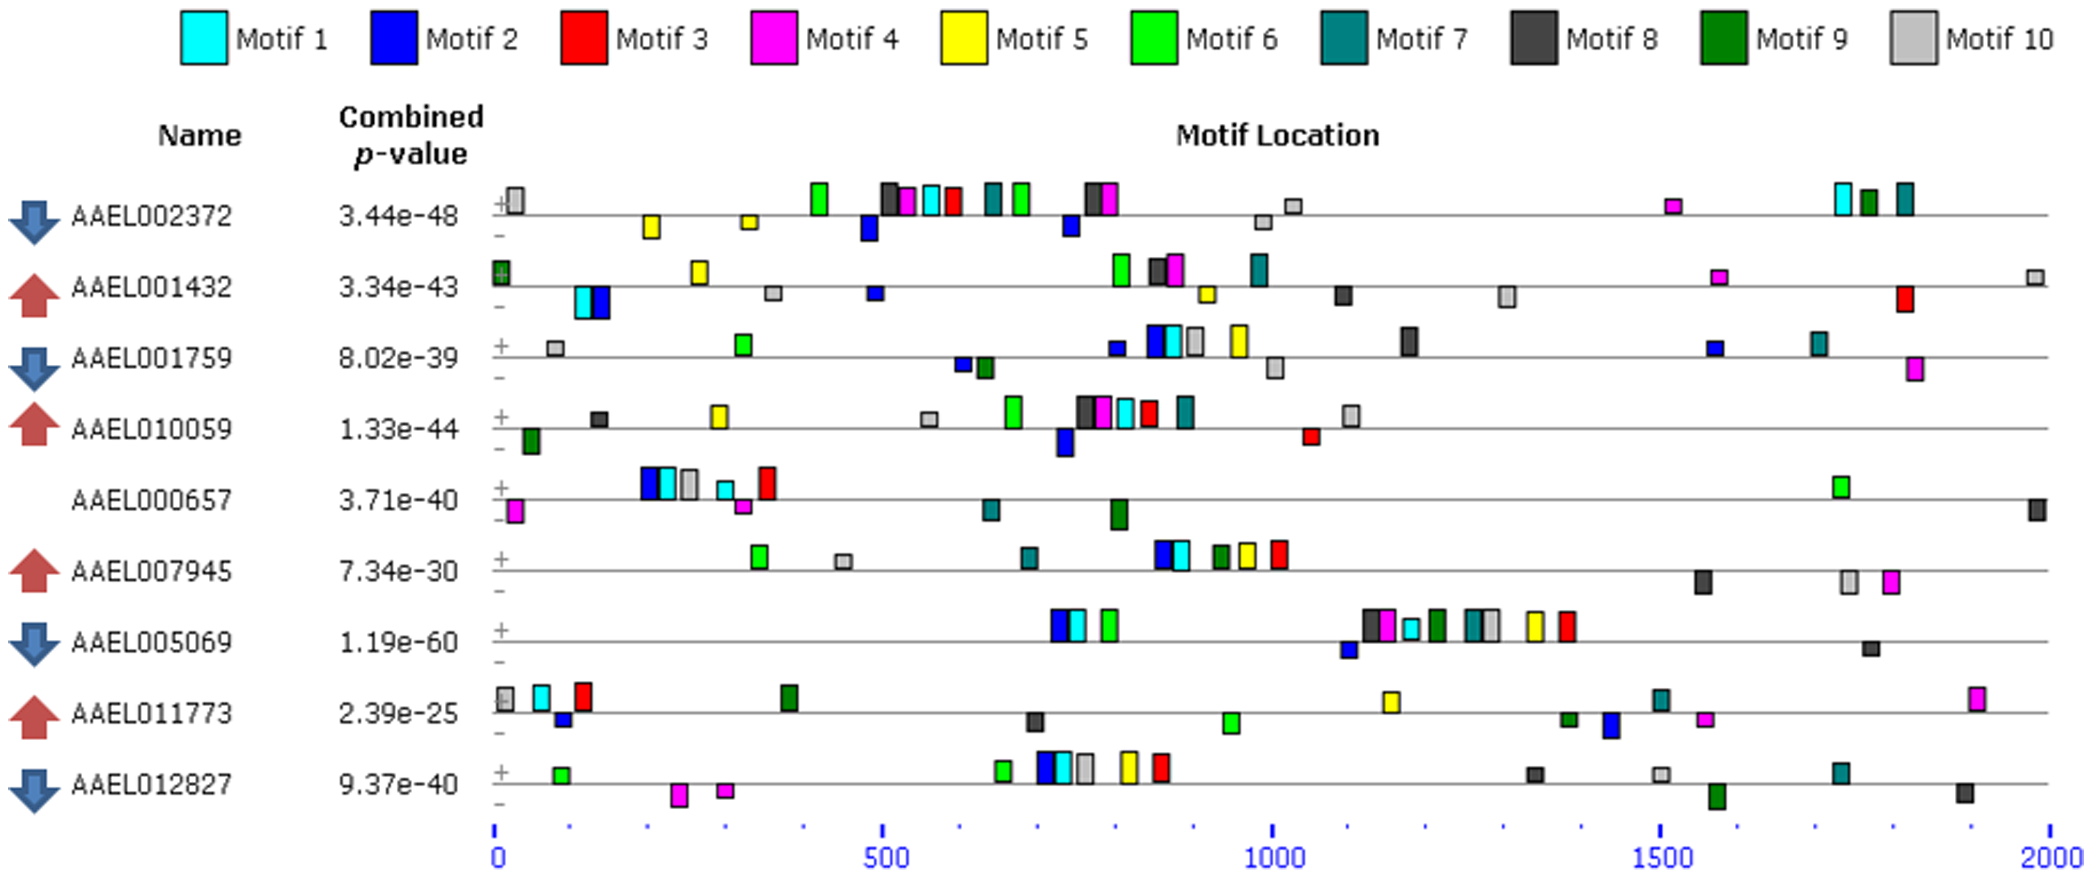
\includegraphics[width=.99\textwidth]{figures/figs/bonizzoni2012complex-cre.png}

\caption[MEME analysis of nine genes with \texorpdfstring{FPKM\textsubscript{DENVI}}{FPKM DENVI} ≥ 100 in carcasses and salivary glands at 14 dpi]{\sf \textbf{MEME analysis of nine genes with \texorpdfstring{FPKM\textsubscript{DENVI}}{FPKM DENVI} ≥ 100 in carcasses and salivary glands at 14 dpi} These genes also were identified with transcripts exhibiting significant differential accumulation in analyses of salivary gland samples of the Liverpool strain infected with DEV2 Thailand 16881 [26]. Colored boxes represent individual putative CREs and their locations in promoters of each gene. Red and blue arrows adjacent to Ensembl Gene ID indicate those genes whose transcripts were detected previously as more or less abundant following DENV infection [26]. Distances in base-pairs are provided below the schematic of each gene.
doi:10.1371/journal.pone.0050512.g004

Excerpted from \cite{bonizzoni2012complex}}
\label{fig:bonizzoni2012complex-cre}
\end{figure}

% \texorpdfstring{FPKM\textsubscript{DENVI}}{FPKM DENVI}

A total of 94 genes had FPKM ≥ 100 in \gls{DENVI} mosquitoes in both carcass and salivary gland samples at 14 \gls{dpi}, with corresponding values in B mosquitoes ≤ 100.
The putative promoter regions of these genes analyzed by MEME revealed the presence of two groups of motifs (Figure \ref{fig:bon2012complex-S5}: motifs 1, 2, 3, 4, 5, 7, 9, 10) co-occurring or alternating in 14 genes associated with diverse functions: AAEL001759 [40S ribosomal protein S9], AAEL005069 [ras-related protein Rab-1A], AAEL002372 [40S ribosomal protein S11], AAEL005165 [chaperone protein DNAj], AAEL000657 [hypothetical protein], AAEL005471 [Sec61 protein complex gamma subunit], AAEL001432 [protein disulfide isomerase], AAEL010059 [bacterial-type ABC transport ATP-binding subunit or RNAse l inhibitor], AAEL013407 [Catalase], AAEL007945 [eIF3 h], AAEL010169 [hypothetical protein], AAEL012827 [endoplasmin], AAEL011773 [calreticulin], AAEL010777 [TRX, putative].
These genes, except for AAEL002372, had high read coverage also in midgut samples, but not necessarily higher or equal accumulation in \gls{DENVI} versus B mosquitoes.
Some of these genes were detected previously as significantly differentially accumulated in the salivary glands of mosquitoes of the \gls{LVP} strain infected with \gls{DENV}2 Thailand 16681 (Figure \ref{fig:bonizzoni2012complex-cre}; \cite{Luplertlop2011}).
Specifically, the transcription products of AAEL001432, AAEL010059, AAEL007945 and AAEL011773 were more abundant in salivary glands of infected \gls{LVP}, while the opposite was observed for AAEL001759, AAEL005069, AAEL002372 and AAEL012827, which were more abundant in uninfected samples.
AAEL00657 was listed as both up- and down-regulated following \gls{DENV} infection, most likely at different time points, but this is not explicit in the report \cite{Luplertlop2011}.
MADS\_MCM1+SFF\_M01051 and bZIP transcription factors were the best matches to motifs 1, 2, 5 and 7 (e-value ≤ $10^{-5}$).
Motif 3 has sequence similarity with motifs 5 and 7 of the previously designated “carcass module” and matches to trp\_AtMYB-84\_M00970 (e-value = $2.25E-10$) and RREB-1 (e-value = $2.16E-7$).
The best match of motif 9 is to the HMG transcription factor ($1.87E-5$).


\subsection{Discussion}

The dengue-susceptible strain \gls{CTM} is well-documented in its ability to disseminate quickly viruses to peripheral tissues when compared to long-established laboratory strains \cite{Salazar2007}.
We describe in \citet{bonizzoni2012complex} changes in transcript accumulation levels in \gls{CTM} during the course of a Jam 1409 \gls{DENV}2 infection.
Our analyses include multiple post-infection time-points and three tissues important for the viral transmission cycle: midguts, salivary glands and carcasses, the latter of which includes the fat body.
The RNA-seq technology used in this study interrogates the whole \Aa\ transcriptome and allows for absolute quantification of poly-adenylated RNA levels.
In general, more depleted rather than enriched transcript accumulation was observed.
Importantly, hundreds of genes had exclusive read-coverage only in \gls{DENVI} mosquitoes, but their accumulation levels were generally low (FPKM$_{DENVI}$ < 4 in carcass and midgut samples and < 15 in salivary gland samples).

The “\gls{DENV} down-regulation” trend is consistent to that observed with the Rockefeller (ROCK) strain infected by \gls{DENV}2 New Guinea in transcriptional responses examined in whole-body (1–2, 7 and 14 \gls{dpi}) or midgut samples (10 \gls{dpi}) and in salivary glands of the \gls{LVP} strain infected with \gls{DENV}2 Thailand 16681 \cite{Xi2008}, \cite{Luplertlop2011}, \cite{Sim2012}, \cite{Colpitts2011}.
These results support the hypothesis that dengue infection has a negative impact on fitness.
However, a larger number of genes had products that increased instead of decreased in abundance in carcass samples 10 \gls{dpi} and in salivary glands at 14 \gls{dpi} in ROCK mosquitoes infected with \gls{DENV}2-New Guinea \cite{Xi2008}, \cite{Sim2012}.
This trend also was evident in \Aa\ Aag2 cultured cells infected by \gls{DENV}2 New Guinea and in both susceptible (Moyo-S) and resistant (Moyo-R) strains infected with \gls{DENV}2 Jam1409 \cite{Sim2010}, \cite{Behura2011}.
These results emphasize the complex relationship among \Aa\ and dengue viruses.



\subsubsection{\textit{Cis}-regulatory Elements}

The preferred promoter for an anti-dengue effector gene would be one that is induced following a bloodmeal and is not affected by viral infection.
Furthermore, we hypothesize that genes with this preferred expression profile may share common regulatory mechanisms based on common \glspl{CRE}.
Analysis of the 5′-end of genes whose transcripts exhibited accumulation profiles exclusively in salivary gland following \gls{DENV} infection did not reveal substantial co-occurrence of \glspl{CRE}.
The regulation of these genes is likely not coordinated through common promoter elements.
In contrast, co-occurring putative \glspl{CRE} were identified for genes whose transcripts were represented and modulated highly in response to dengue infection in midguts (1–4 \gls{dpi}), carcasses (all time points studied) and salivary glands and carcasses (14 \gls{dpi}).

Several of the identified motifs showed high-quality matches to known transcription factors.
The \glspl{CRE} likely are not related specifically to dengue infection since the majority of the genes included in the analyses also had read coverage in B mosquitoes.
This observation does not affect the potential utility of the \glspl{CRE} as components of synthetic promoters to direct expression of anti-dengue effector molecules.
Indeed, driving effector gene expression with control DNA that responds to an uninfected bloodmeal and either is unaffected or is enhanced by an infected bloodmeal could elicit a protective antiviral response in the mosquitoes.
Remarkably, 10 genes whose transcripts were modulated following \gls{DENV}2 16881 infection in \gls{LVP} salivary gland samples were among the 14 genes with FPKM$_{DENVI}$ ≥ 100 in our carcass and salivary gland samples that have a common group of \gls{CRE} motifs \cite{Luplertlop2011}.
However, not all of these ten genes had transcripts that were consistently more abundant following infection, and one gene, (AAEL00657), had transcripts reported as more and less abundant \cite{Luplertlop2011}.
These results and the findings that several motifs are putative binding sites for transcription factors acting through repressors and activators support a complex model of transcription modulation that requires further investigation.

\subsection{Conclusions}

Dengue fever is the most important arboviral disease world-wide, with \Aea\ being the major vector.
Interactions between the mosquito host and dengue viruses (\gls{DENV}) are complex and vector competence varies among geographically-distinct \Aa\ populations.
Additionally, dengue is caused by four antigenically-distinct viral serotypes (\gls{DENV}1–4), each with multiple genotypes.
Each virus genotype interacts differently with vertebrate and invertebrate hosts.
Analyses of alterations in mosquito transcriptional profiles during \gls{DENV} infection are expected to provide the basis for identifying networks of genes involved in responses to viruses and contribute to the molecular-genetic understanding of vector competence.
In addition, this knowledge is anticipated to support the development of novel disease-control strategies.
RNA-seq technology was used to assess genome-wide changes in transcript abundance at 1, 4 and 14 days following \gls{DENV}2 infection in carcasses, midguts and salivary glands of the \Aa\ Chetumal strain.
\gls{DENV}2 affected the expression of 397 \Aa\ genes, most of which were down-regulated by viral infection.
Differential accumulation of transcripts was mainly tissue- and time-specific.
Comparisons of our data with other published reports reveal conservation of functional classes, but limited concordance of specific mosquito genes responsive to \gls{DENV}2 infection.
These results indicate the necessity of additional studies of mosquito-\gls{DENV} interactions, specifically those focused on recently-derived mosquito strains with multiple dengue virus serotypes and genotypes.


The study of genome-wide changes in transcript abundance in \Aa\ following dengue infection is anticipated to identify genes and control DNA elements involved in vector competence.
This knowledge is expected to contribute to development of novel vector control strategies.
The interactions between the mosquito host and the virus are complex at both the individual and population levels.
Many mosquito tissues are affected by the virus during the course of the infection and \Aa\ strains can show unique responses of the transcriptome in response to a bloodmeal and susceptibility to \gls{DENV} infection \cite{Black2002}, \cite{bonizzoni2012strain}.
Additionally, the variation in \gls{DENV} serotypes and genotypes contributes to genetically-distinct differences in vector competence \cite{Anderson2006}, \cite{Weaver2009}.
While we identified modulations in transcript abundance following \gls{DENV} infection that represent genes encoding similar functional categories, a limited number of specific genes were concordant across the mosquito strains and \gls{DENV}2 genotypes following comparison of our data with previous studies \cite{Xi2008}, \cite{Luplertlop2011}, \cite{Behura2011}, \cite{Sim2012}, \cite{Colpitts2011}.
Furthermore, the direction of changes in transcript abundance in samples from infected and uninfected mosquitoes was not always conserved among the various studies, an observation that we consider independent of the methodology used to assess differential transcript accumulation.
These results support the need for a comprehensive analysis of dengue infection focusing on recently-colonized laboratory strains or wild-caught mosquitoes to capture most of the genetic variability at the host level and different \gls{DENV} serotypes/genotypes \cite{Armstrong2001}.
This analysis also should account for possible variation in the progression of the viral infection and timing of host gene expression.



\pagebreak
\section{Strain variation in the transcriptome of the dengue fever vector, \Aea. \cite{bonizzoni2012strain}}
%\todo[inline]{import text for STRAIN VARIATION}





Studies of transcriptome dynamics provide a basis for understanding functional elements of the genome and the complexity of gene regulation.
The dengue vector mosquito, \Aea, exhibits great adaptability to diverse ecological conditions, is phenotypically polymorphic, and shows variation in vectorial capacity to arboviruses.
Previous genome sequencing showed richness in repetitive DNA and transposable elements that can contribute to genome plasticity.
Population genetic studies revealed a varying degree of worldwide genetic polymorphism.
However, the extent of functional genetic polymorphism across strains is unknown.
The transcriptomes of three \Aa\ strains, \gls{CTM}, \gls{Rex-D} and \gls{LVP}, were compared.
\gls{CTM} is more susceptible than \gls{Rex-D} to infection by dengue virus serotype 2.
A total of 4188 transcripts exhibit either no or small variation (< 2-fold) among sugarfed samples of the three strains and between sugarfed and bloodfed samples within each strain, corresponding most likely to genes encoding products necessary for vital functions.
Transcripts enriched in bloodfed mosquitoes encode proteins associated with catalytic activities, molecular transport, metabolism of lipids, carbohydrates and amino acids, and functions related to blood digestion and the progression of the gonotropic cycle.
Significant qualitative and quantitative differences were found in individual transcripts among strains including differential representation of paralogous gene products.
The majority of immunity-associated transcripts decreased in accumulation after a bloodmeal and the results are discussed in relation to the different susceptibility of \gls{CTM} and \gls{Rex-D} mosquitoes to \gls{DENV2} infection.

This mosquito species is phenotypically polymorphic, has great adaptability to diverse ecological conditions, and shows variation in vectorial capacity for arboviruses \cite{Bennett2002,Black2002,Kuno2010}.
Genetic polymorphism among geographically distinct \Aa\ populations is documented \cite{Urdaneta-Marquez2011}; however, the extent of genome sequence polymorphism and its effects on transcriptional activity are not known.

The transcriptional profiles of three \Aa\ strains, \gls{LVP}, \gls{CTM}, \gls{Rex-D}, were investigated.
\gls{LVP} originated in West Africa in the 1930s, and its genome is sequenced \cite{Nene2007}, \gls{CTM} was derived from the Yucatan Peninsula in Mexico in the early 2000s \cite{Bennett2002,Gubler1985,Richardson2006a}, whereas \gls{Rex-D} was established from mosquitoes captured in Puerto Rico in the early 1990s \cite{Miller1991}.
\gls{CTM} supports a faster and more intense dissemination of \gls{DENV2} than \gls{Rex-D} \cite{Bennett2002,Salazar2007}.
Our data show significant differences in transcript accumulation among strains, and the results may account for the differing susceptibility of \gls{CTM} and \gls{Rex-D} mosquitoes to virus infection.


\subsection{Results}
\subsubsection{RNA-seq mapping summary}

Transcriptional profiles of \gls{LVP}, \gls{CTM}, and \gls{Rex-D} strains before and after a bloodmeal were compared.
RNA-seq libraries were generated with the use of RNA extracted from females collected 3 to 5 days after eclosion and kept either on a sugar diet (S) or harvested 5 h \gls{PBM} (B) (not shown).
Two RNA-seq libraries were constructed for each RNA sample.
The reproducibility of the parallel libraries was verified (not shown), and the data from the two technical replicates were merged for further analyses.
Reads mapping to multiple genomic locations were discarded during Bowtie alignment \cite{Langmead2009}.
As a consequence, the accumulation levels of transcripts encoded by highly conserved gene families are under-estimated.
This bias is expected to affect all samples equally; therefore, if the absolute accumulation level of a transcript is underestimated, differences across conditions still can be calculated.



\subsubsection{Constitutively accumulated transcripts}

A total of 4188 transcripts exhibit no or small variation (≤ 2-fold) among S samples of the three strains and between B and S samples within each strain and correspond most likely to genes that encode products necessary for vital and/or basal metabolic functions (not shown).
Function−parent attributions for this group of transcripts revealed a predominance of those encoding proteins with binding activity over transcripts with molecular function and catalytic activity (not shown).
Functional description is available for 2262 of these 4188 transcripts \cite{Lawson2009} (not shown).
More than 10 transcripts were found associated with each of the following classes: protein recycling (ubiquitin and proteasome), zinc finger proteins, WD-repeat proteins associated with diverse functions (i.e. RNA-processing complexes, transcription, cytoskeleton assembly), ribosome proteins, signal transduction (GTP binding proteins, G coupled proteins), redox processes (cytochrome), translation (eukaryotic translation initiation factor), transcription (transcription factors, mediator complex), membrane trafficking (rab), cell growth, differentiation and survival (ras), and immunity (PIWIs, autophagy proteins, galectins, TOLL, IMD, and JACK-STAT pathway signaling members).


Approximately 25\% of all analyzed transcripts accumulated differentially in S mosquitoes of different strains.
However, in the majority of cases the differences observed were lower than 2-fold (not shown).
Here is described only differences between the DEN-refractory \gls{Rex-D} and the more permissive \gls{CTM} strain.
Totals of 2992 and 2080 transcripts accumulated more in \gls{Rex-D} or \gls{CTM}, respectively.
Six were accumulated more than 5-fold in \gls{CTM} with respect to \gls{Rex-D}, including four of unknown function, one (AAEL005534-RA) annotated as a gonadotropin-inducible transcription factor, and one (AAEL014188-RA) annotated as a serine-type endopeptidase.
In contrast, 310 transcripts accumulated ≥ 5-fold in \gls{Rex-D} with respect to \gls{CTM}.
Functions could be attributed to 51\% of these and they include aldehyde oxidases, cytochrome P450s, G-coupled receptors, N-acetylgalactosaminyltransferases, and nicotinic acetylcholine receptors.
Immunity-associated transcripts accumulated differently in \gls{CTM} and \gls{Rex-D} S mosquitoes include five C-type lectins (AAEL008681-RA [CTL12], AAEL012353-RA [CTL15], AAEL005482-RA [CTL18], AAEL013566-RB [CTLGA2], AAEL017484-RA [CTLGA4]), two heme peroxidases (AAEL00376-RA [HPX4], AAEL002354-RA), one class B scavenger receptor (AAEL010655-RA [SCRBSP2]), a fibrinogen-related protein (AAEL008646-RA [FREP10]), and a Toll-like receptor (AAEL000671-RA [TOLL6]).


Quantitative reverse transcriptase, gene amplification, i.e., polymerase chain reaction (qRT-PCR) was performed on a selection of 13 transcripts and RNA from \gls{CTM}, \gls{Rex-D}, and \gls{LVP} mosquitoes.
The qRT-PCR results validated the RNA-seq data, with only two exceptions (transcript AAEL011871-RA in \gls{CTM} and AAEL008848-RA in \gls{Rex-D}; not shown).
To assess the similarity of the RNA-seq data with the qRT-PCR measurements, we calculated Pearson correlations of 0.97 (p < 0.001), 0.85 (p < 0.001), and 0.90 (p < 0.01) for \gls{LVP}, \gls{CTM}, and \gls{Rex-D}, respectively.
T-test values were 2.18 (p = 0.148), 2.18 (p = 0.453), and 2.18 (p = 0.188), respectively, for the three strains (not shown).

The accumulation of 1845 and 981 transcripts consistently increased and decreased, respectively, in all three strains after a bloodmeal (not shown).
In general, \gls{Rex-D} exhibited the lowest fold-changes and the smallest number of transcripts accumulated highly after the bloodmeal (not shown).
This observation supports the interpretation that \gls{CTM} mosquitoes respond quicker or more intensively to a bloodmeal than \gls{LVP} and \gls{Rex-D}.
To test this hypothesis, the expression profiles of five transcripts were analyzed by qRT-PCR at 5, 8, 12, and 24 h \gls{PBM}.
Results for four of the five transcripts tested showed a greater response of \gls{CTM} to a bloodmeal compared with mosquitoes of the other two strains (not shown).




Despite the observation that the same functional classes are represented within groups of transcripts that increased and decreased in accumulation after a bloodmeal, the numbers of transcripts associated with the various functions differed significantly (not shown).
The transcripts accumulated after a bloodmeal were enriched in functions related to protein-turnover and chaperones, transcription, translation, posttranslational modification, and RNA processing.
These transcripts encode proteins associated with catalytic activities, in transport and metabolism of lipids, carbohydrates and amino acids, and related to blood digestion and the progression of the gonotropic cycle.
Many of the transcripts showing the greatest decrease in accumulation after a bloodmeal in all three strains encode structural proteins.

The number of strain-specific transcripts varying highly (< 10-fold) in abundance between B and S mosquitoes is smaller in general than those found in all three strains (not shown).
\gls{CTM} mosquitoes show both the greatest number of strain-specific, differentially accumulated transcripts (not shown) and the largest range of changes in transcript accumulation levels.
Overall, the largest proportion of transcripts showing strain-specific increased accumulation after bloodmeal are linked to binding and catalytic functions and associated with transcription, translation, and posttranslational modification, whereas the largest proportion of strain-specific decreased transcripts are linked to transcription, translation, posttranscriptional modification, and RNA processing in \gls{LVP} and \gls{CTM} and to transport and metabolism of lipids, carbohydrates, and amino acids in \gls{Rex-D} (not shown).


\subsubsection{Protein network analysis of bloodmeal-induced changes in transcript accumulation}

By using a Markov Cluster algorithm, \cite{Guo2010} developed a protein interaction network in which 3500 \Aa\ proteins are organized into 494 functional modules.
A total of 2465 of these proteins are encoded by transcripts exhibiting significant differential accumulation between B and S mosquitoes in at least one of the three strains analyzed (not shown).
Modules enriched in Gene Ontology terms for cytoplasm organization and biogenesis, ribosome biogenesis and assembly, transcription, DNA metabolic processes, response to endogenous stimuli, and cell cycle were enriched significantly with proteins encoded by transcripts increased in accumulation in all three strains after a bloodmeal (not shown).
A module enriched in Gene Ontology terms for cytoskeleton organization and biogenesis, reproduction, and cell differentiation was enriched significantly with proteins corresponding to transcripts consistently decreased in accumulation following a bloodmeal.
Results from the protein network analyses are consistent with those from functional attribution of the differentially accumulated transcripts.

\subsubsection{Metabolic pathways involving transcripts differentially accumulated post-bloodmeal}

\begin{figure}[h]

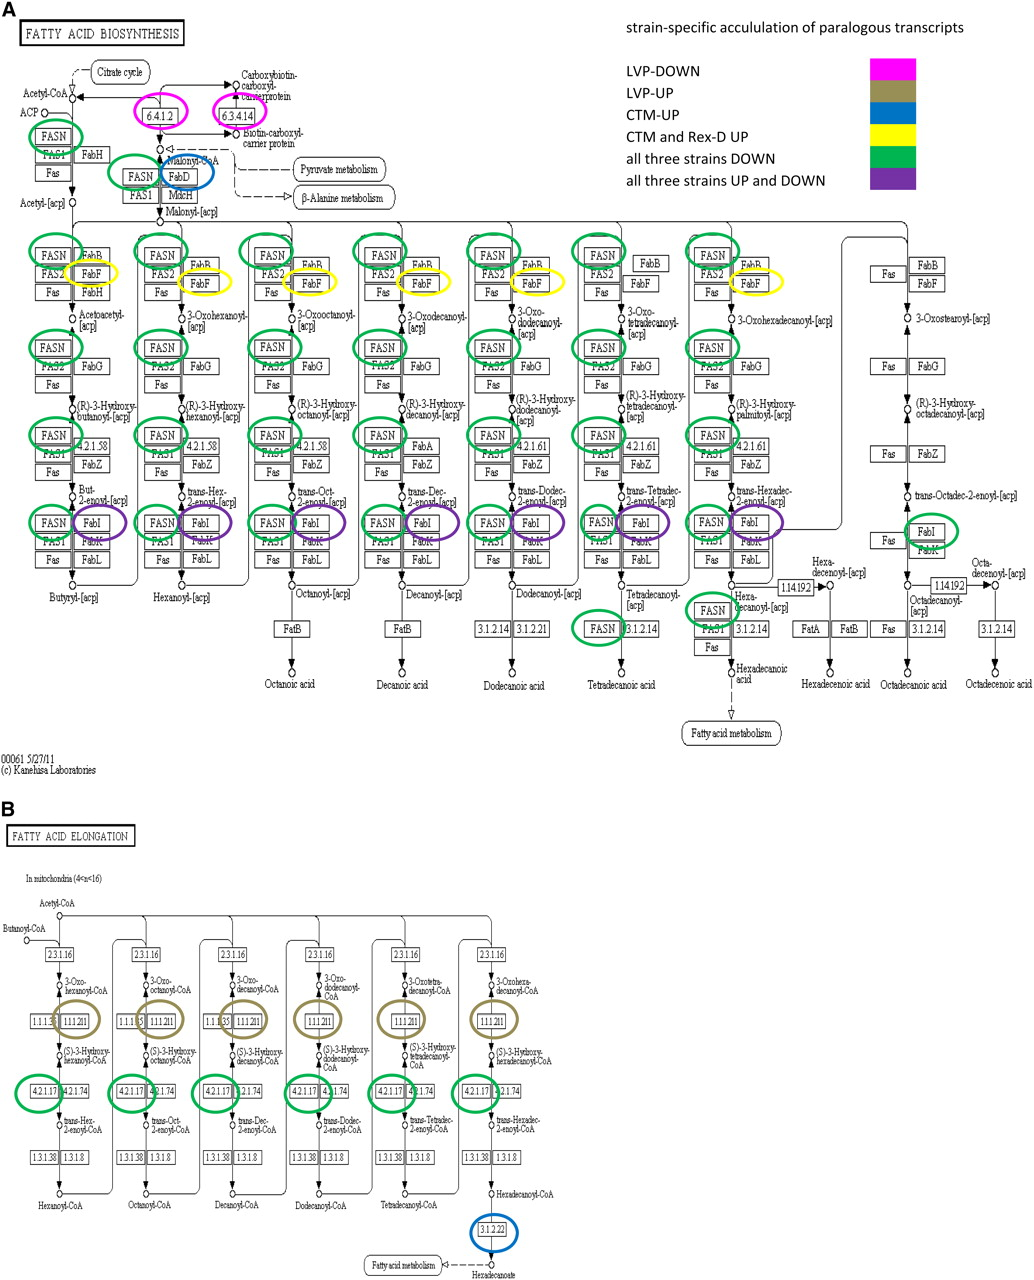
\includegraphics[width=.9\textwidth]{figures/figs/aa-diff-paralogs.jpg}

\caption[Fatty acid biosynthesis and elongation in mitochondria]{\sf \textbf{Fatty acid biosynthesis and elongation in mitochondria:} Proteins corresponding to transcripts accumulated in a strain-specific manner are circled in a color corresponding to the strain and condition defined in the legend (panels A and B).

Excerpted from \cite{bonizzoni2012strain}}
\label{fig:aa-diff-paralogs}
\end{figure}

Metabolic pathways correlated with transcripts increased in accumulation after a bloodmeal in all three strains were visualized in LinkinPath \cite{Ingsriswang2011} alongside pathways associated with transcripts accumulated in a strain-specific manner and transcripts decreased in accumulation after a bloodmeal (not shown).
As seen with the function−parent attribution analyses, the transcripts increased and decreased in accumulation are associated with proteins involved in similar pathways.
However, differential expression of paralogous genes among the strains was observed that could account for the intensity and/or the rate of pathway activation/deactivation after a bloodmeal.
For example, biosynthesis of fatty acids associates predominantly with transcripts decreased in accumulation in all three strains after a bloodmeal, but the elongation of fatty acids in mitochondria was exclusively associated with transcripts increased in accumulation (Figure \ref{fig:aa-diff-paralogs}).
Proteins corresponding to transcripts accumulated differentially in a strain-specific manner were identified in both cases, with the same protein function encoded by paralogous transcripts in the different strains.
Examples include FabI (enoyl-[acyl carrier protein] reductase) of the fatty acid biosynthesis pathway linked to transcripts AAEL003961-RA and AAEL002493-RA, which significantly increased in all three strains (fold-changes: 1.4-2.4); AAEL009634-RC and AAEL014840-RA, both of which increased 2-fold in \gls{CTM}; AAEL000705-RA, AAEL000689-RA and AAEL004273-RA, which decreased in \gls{CTM} (fold-changes: 2.5-4.4); AAEL009685-RB, which decreased 5.4-fold in \gls{Rex-D}; and AAEL017302-RA, AAEL007669-RA, AAEL008227-RA, AAEL009625-RA, AAEL013491-RA, AAEL017320-RA, AAEL000690-RA, AAEL002228-RA, AAEL003148-RA, AAEL003183-RA, AAEL010075-RA, AAEL012400-RA, and AAEL008016-RA, which decreased in all three strains, with fold-changes in the range of 0.6-11.3.
All of these transcripts are annotated currently as short-chain and steroid dehydrogenases, oxidoreductases, or fatty acid synthases \cite{Ribeiro-AegyXcel} and match to short-chain dehydrogenases in the PFAM database \cite{Finn2008}, with the exception of AAEL002228-RA, whose best match is ketoacyl synthase.
They all have the PKS\_KR enzymatic domain as a best match in the SMART database \cite{Letunic2009}, except for AAEL012400-RA, which matches the SEP enzymatic domain.
The protein HADHA (4.2.1.17 in the fatty acid elongation pathway), functioning as an aldehyde reductase and enoyl-coA hydratase, is associated with transcripts AAEL010146-RB (annotated as 3-hydroxyacyl-coa dehydrogenase) and increased 2.9-fold in \gls{LVP} and AAEL003993-RA (putative cyclohex-1-ene-1-carboxyl-CoA hydratase), which increased in all three strains with fold-changes ranging between 1.6 and 2.3.


Another example of differential accumulation of transcripts representing paralogous genes is seen in the lipase gene family.
Three genes (AAEL001837, AAEL007055, AAEL14551) of the 72 annotated currently as lipases correspond to transcripts accumulated differentially after a bloodmeal in all three strains (fold-changes: −7.5 to 4.3) and eight to transcripts accumulated differentially in a strain-specific manner.
Two (AAEL002909-RA, AAEL001076-RA) of these latter transcripts were found exclusively in S and one (AAEL006970-RA) only in B \gls{CTM} mosquitoes.
The remaining had fold-changes ranging from −2.2 to 2.6.
No reads were mapped in any sample for 21 lipase genes, which may indicate that they are expressed exclusively in adult males or during pre-adult stages of \Aa\ development.
Alternatively, these predicted genes could be pseudogenes.



\subsection{Discussion}
The results reported here reveal that the transcriptomes of \Aa\ mosquitoes from distinct strains vary significantly in complexity and abundance of specific transcripts.
This variation is evident in non-bloodfed mosquitoes and is enhanced after a bloodmeal.
\gls{CTM} showed a larger number of differentially abundant transcripts after a bloodmeal and a wider range of fold-changes than \gls{Rex-D} and \gls{LVP}.


Transcripts associated with metabolism and transport of lipids, carbohydrate and amino acids, and the progression of the gonotropic cycles were among the most increased in accumulation after bloodmeal.
Transcripts decreased most in accumulation after a bloodmeal are associated with structural components.
Transcripts attributed functions in transcription, translation, and posttranslational protein modification also were highly differentially-accumulated, but many of these show strain-specific regulation.
These observations support the hypothesis that important differences among the strains are conferred by distinct patterns of gene expression, protein synthesis and modifications.
Strain differences also may result from selective expression of paralogous transcripts.


Digestion and immunity share bio-products such as \gls{ROS} \cite{Molina-Cruz2008}, and these processes are linked at the protein network level \cite{Guo2010}.
The majority of immunity-related genes were decreased in accumulation in all three strains after a bloodmeal.
The most pronounced decrease in accumulation was observed for the antimicrobial peptide \gls{AMP} (AAEL003389-RA).
Indeed, all AMPs decreased in accumulation with the exception of CecF (AAEL000625-RA), which significantly increased in accumulation exclusively in \gls{CTM}.
The overall AMP decrease may be associated with an increase in bacterial proliferation observed after a bloodmeal \cite{Oliveira2011}.
The most common midgut bacteria do not show proteolysis activity but are implicated in the lysis of red blood cells, which release hemoglobin \cite{Gaio2011}.
At the same time, hemoglobin negatively affects ROS production in the midgut, which triggers bacteria proliferation \cite{Oliveira2011}.
Although ROS reduction potentially favors DEN infection \cite{Oliveira2011}, bacteria proliferation antagonizes it \cite{Xi2008}.
Antioxidant activity by peroxidase and superoxide-dismutase varied across strains.
\gls{CTM} showed the greatest number of transcripts associated with antioxidant activity accumulated after a bloodmeal among the strains analyzed.
In addition, S \gls{CTM} mosquitoes accumulate greater levels of transcripts associated with antioxidant activity than \gls{Rex-D}.
\gls{CTM} also had the largest number of P450 and glutathione-s transferase transcripts accumulated differentially after a bloodmeal, with increases in accumulation up to 15-fold (AAEL000325-RA).
These results support a model of more intense antioxidant activity in B \gls{CTM} than in \gls{Rex-D}, which may facilitate DENV infection in the former.

Transcripts encoding proteins associated with autophagy, IAPs, IMD pathway, and SRRP members represent immunity genes that showed an exception to the overall decline in corresponding-transcript accumulation after a bloodmeal.
Increases were overall within 2-fold.
A notable exception is the IMD pathway member Caspar1 (AAEL014734-RA) that increased 4.7- to 5.8-fold in all strains.
Caspar is a negative regulator of the IMD pathway \cite{Kim2006caspar}; therefore, its up-regulation is consistent with the observed decrease in accumulation of AMPs.

In summary, the \Aa\ strains analyzed demonstrated variability in their transcriptomes before and after bloodmeal.
Profiles differ in the number of transcripts detected, their level of accumulation in S mosquitoes, and in the changes in accumulation following the ingestion of a bloodmeal.
Although these differences may result from distinct RNA turnover rates among strains, it is most likely a result of differential gene regulation.
These data indicate the need for caution in making generalizations about individual gene expression profiles across different strains of \Aa.
For example, constructs used in genetics-based strategies of vector control would require the previous analyses of cross-strain promoter activity \cite{James2011}.
The differences observed encompass several transcripts associated previously with vectorial capacity to DENV.
Future studies will investigate the transcriptomes of \gls{CTM} and \gls{Rex-D} mosquitoes infected with \gls{DENV2}.
Also, it will be necessary to assess the susceptibility of \gls{CTM} and \gls{Rex-D} to other DENV serotypes to determine whether or how their distinct transcriptional responses to bloodmeals described herein influence vector competence.




%%% Local Variables: ***
%%% mode: latex ***
%%% TeX-master: "thesis.tex" ***
%%% End: ***
